\section{Photometric reduction of CCD images} \label{sec:photoreduction}


An image obtained by a telescope using a CCD camera is called a raw image. A raw image is affected by before mentioned defects and noises. Therefore, the image needs to be corrected to a certain level to obtain precise photometric results \cite{articleParimucha}. This process is called image calibration, which contains several steps discussed here below.  

\subsection{Calibration images}
The image calibration consists of three steps: subtraction of BIAS image, subtraction of DARK image and division by FLAT FIELD image.

    %%%%%%%%%%%%%%%%%%%%%%%%%%%% 
    \subsubsection{BIAS frame}
    As mentioned earlier, to solve an issue with negative values in ADC, bias voltage was introduced.
    However, during photometry, the offset bias value needs to be subtracted from the image to achieve correct values. To retrieve the bias values on the pixels, the BIAS frame is created. 
    The aim is to retrieve an image without any residual signal in the pixels originating from the camera. This is achieved by taking an image with a closed shutter and zero exposure time \cite{articleParimucha}.
     
             
    %%%%%%%%%%%%%%%%%%%%%%%%%%%%   
    \subsubsection{DARK frame} 

    DARK frames are introduced to detect dark current in the image. Apart from that, they are also capable of detecting hot and dead pixels on the image. 
    To create a DARK frame, an image is taken with a closed shutter to eliminate photo-electrons from stars and the sky. Values in the pixels are from the dark current and bias voltage. Therefore to obtain a correct DARK frame, bias values need to be subtracted from the DARK frame. 
    As mentioned before, dark current is proportional to chip temperature and exposure time. This implies that in order to have correct dark current values, the DARK frame needs to be taken with the same exposure time as the raw image. The same goes for the temperature of the CCD chip \cite{articleParimucha} \cite{articleCcdOnline} \cite{phy217}. 
    

    %%%%%%%%%%%%%%%%%%%%%%%%%%%%  
    \subsubsection{FLAT FIELD frame} 
    
    Taking an image of the perfectly uniform light source, would not result in an image with the same amount of counts in each pixel. Readout noise, bias voltage, and dark current are all contributing to this fact. However, even without them, the image would not be uniform. The main reason is the sensitivity of each pixel. Due to the manufacturing limitations, no two pixels convert the light photons into electrons the same way \cite{articleCCDartifacts} \cite{phy217}.
    
    The solution to this problem is by taking a FLAT FIELD frame, which corrects pixel to pixel sensitivity. As mentioned before, the frame is created by taking a picture of an evenly illuminated field. One of the most common ways is to take an image of the twilight sky.
    Similarly, as with the DARK frame, this FLAT FIELD frame contains values from bias voltage as well as dark current. To get a single correct FLAT FIELD frame, these values need to be subtracted.
    Another great feature of the FLAT FIELD frame is that it can also detect dust particles on the filters and lenses. These manifest as dark rings on the image. They are the same with different exposure times but vary from filter to filter. However, they also differ from time to time as some particles can be shifted, eliminated, or added. 
    Furthermore, flat fielding can clear dimming on the edge of the image. This is also called vignetting and is caused by out-of-focus obstructions in the light path \cite{articleParimucha} \cite{phy217}.
    
    After taking the FLAT FIELD frame, signal values are arbitrary, since it only means how bright the source of illumination was. The important part is the differences in the signal across the chip. FLAT FIELD frame is therefore normalized in a way that the average signal in each pixel is 1 \cite{phy217}.
    %% najst citaciu tohto
    
        
    %%%%%%%%%%%%%%%%%%%%%%%%%%%%  
    \subsubsection{MASTER frame}
    
    Due to the nature of reading the image from the CCD chip, every calibration image contains readout noise, which can cause issues during the calibration process. To minimize the noise, multiple calibration images are taken, which are then reduced to one MASTER frame. 
    The MASTER frame is created by taking average or median values of the pixel from the multiple calibration images (BIAS, DARK, FLAT FIELD).
    After the process, we have MASTER BIAS, MASTER DARK, and MASTER FLAT FIELD frames (shown in the Figure \ref{fig:masterframes}), and these are later used in photometric reduction \cite{articleParimucha}.
   
   
   
    \begin{figure}[!h]
    \centering
        \begin{subfigure}[t]{.3\textwidth}
            \centering
            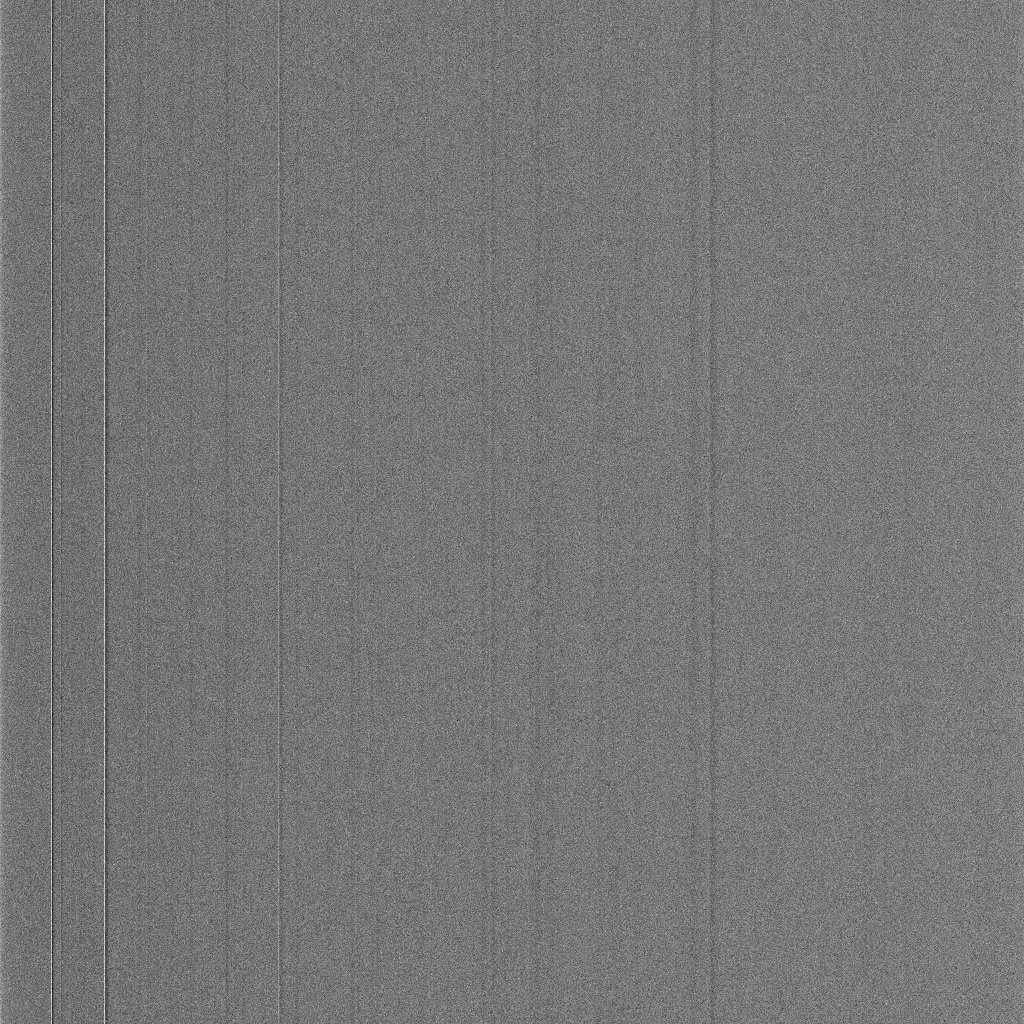
\includegraphics[width=\textwidth]{images/biasframe.jpg}
            \caption{MASTER BIAS frame.}
            \label{fig:biasframe}
        \end{subfigure}
        \hfill
        \begin{subfigure}[t]{.3\textwidth}
            \centering
            
\includegraphics[width=\textwidth]{images/dark90s.jpg}
            \caption{MASTER DARK frame with exposition time of 90 seconds.}
            \label{fig:darkframe}
        \end{subfigure}
        \hfill
        \begin{subfigure}[t]{.3\textwidth}
            \centering
            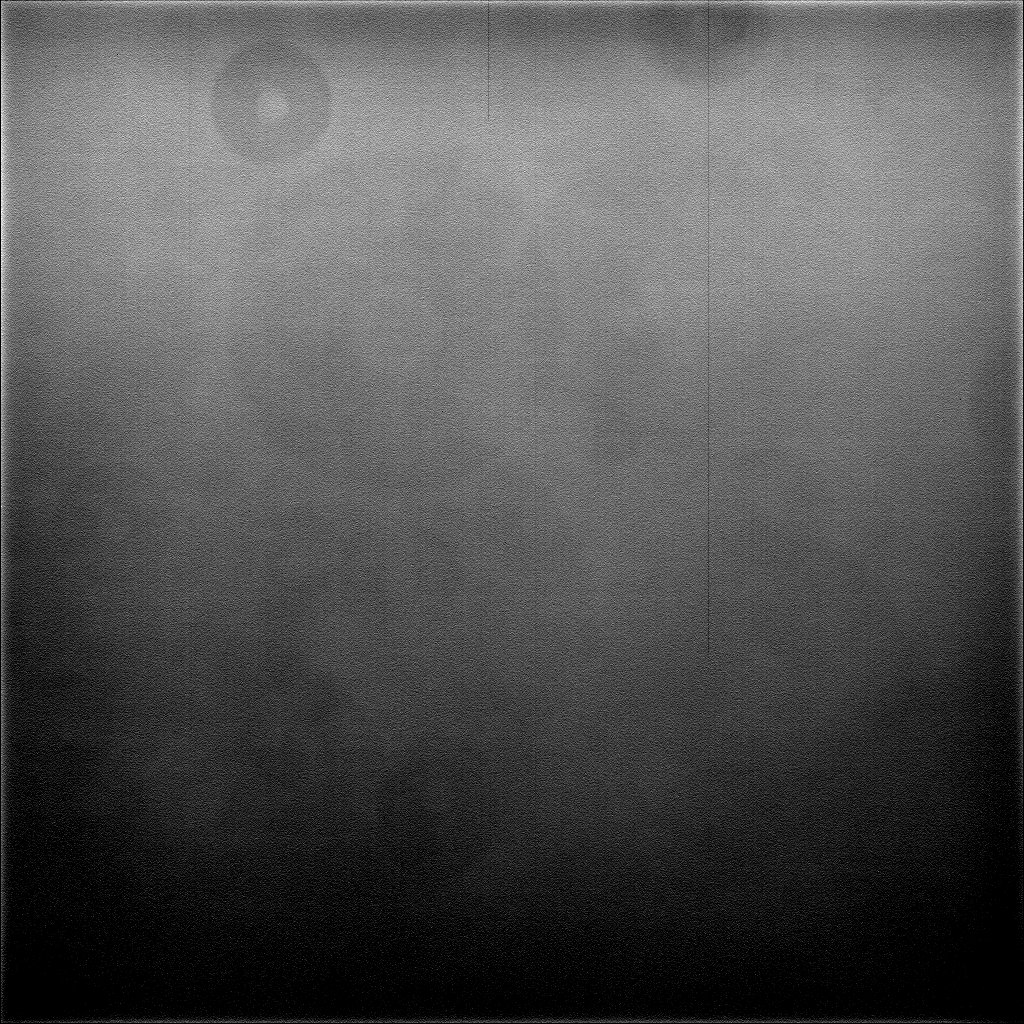
\includegraphics[width=\textwidth]{images/flatframe.jpg}
            \caption{MASTER FLAT FIELD frame.}
            \label{fig:flatframe}
        \end{subfigure}
        \hfill
        \caption{Examples of MASTER frames acquired by AGO in Modra.}
        \label{fig:masterframes}
    \end{figure}



\subsection{Formal definition}

The intensity of the raw image at the pixel $(x,y)$, with exposure time $t$ and temperature of CCD chip $T$ can be generally written as
\[ I(x,y,t,T) = b(x,y,T) + d(x,y,t,T) + i(x,y,t,T) f(x,y,t_f,T) \]

where $b(x,y,T)$ is the intensity of BIAS frame. Exposure time is ommited since the BIAS frame is taken with exposure time of zero. Intensity of DARK frame is denoted as $d(x,y,t,T)$. $f(x,y,t_f,T)$ is the response factor of FLAT FIELD frame, taken with exposure time $t_f$ \cite{articleParimucha}.

The intensity of the real object, which we want to obtain is denoted as $i(x,y,t,T)$. 
All the images are dependent on temperature $T$, which can be omitted from the equation since the CCD chip is cooled down and images are usually taken with the same temperature \cite{articleParimucha}.

To get the real intensity of the object the previous equation becomes
\[
i(x,y,t) = \frac{ I(x,y,t) - b(x,y) - d(x,y,t)}{f(x,y,t_f)}
\]
